\begin{figure*}[!ht]
    \centering
    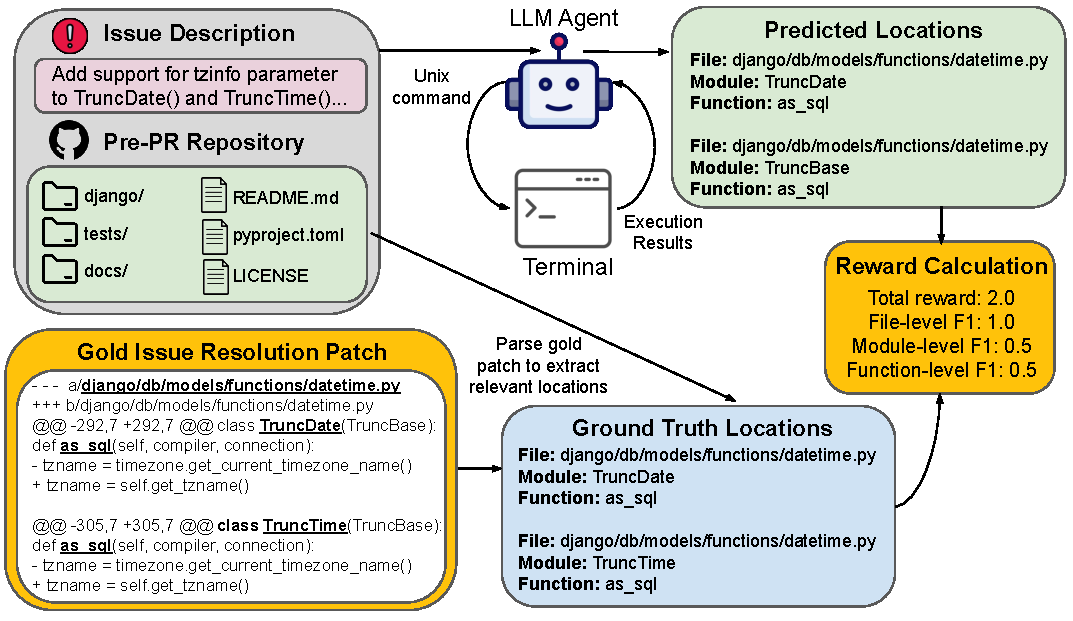
\includegraphics[width=0.71\textwidth]{Figures/sys_diagram_new_cropped (2).pdf}
    \caption{An overview of \methodname: given an issue, the agent navigates the pre-PR codebase using a terminal and predicts the relevant files, modules, and functions. The reward function computes F1 scores for these three granularities using ground truth locations extracted from the gold issue resolution patch.}
    \label{fig:system_diagram}
    \Description{System diagram illustrating the CodeScout recipe. The diagram shows an agent exploring a codebase using a terminal to predict relevant files, modules, and functions based on a given GitHub issue. The reward calculation is shown to the right that computes F1 scores for these predictions using ground truth locations extracted from the issue resolution patch.}
\end{figure*}

% \begin{wrapfigure}{r}{0.6\textwidth}
%     \centering
%     \vspace{-10pt} % optional: adjust vertical spacing
%     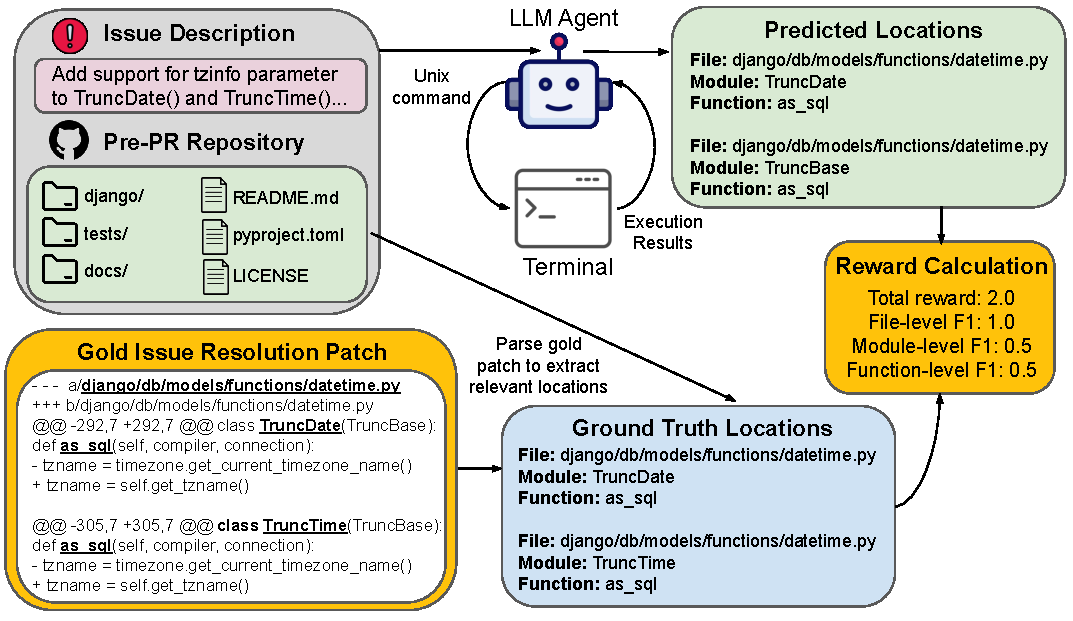
\includegraphics[width=0.6\textwidth]{Figures/sys_diagram_new_cropped (2).pdf}
%     \caption{An overview of \methodname: given an issue, the agent navigates the pre-PR codebase using a terminal and predicts the relevant files, modules, and functions. The reward function computes F1 scores for these three granularities using ground truth locations extracted from the gold issue resolution patch.}
%     \label{fig:system_diagram}
%     \vspace{-10pt} % optional: adjust spacing below
% \end{wrapfigure}